%
% File acl2012.tex
%
% Contact: Maggie Li (cswjli@comp.polyu.edu.hk), Michael White (mwhite@ling.osu.edu)
%%
%% Based on the style files for ACL2008 by Joakim Nivre and Noah Smith
%% and that of ACL2010 by Jing-Shin Chang and Philipp Koehn

\documentclass[11pt,a4paper]{article}
\usepackage[hyperref]{naaclhlt2018}
\usepackage{times}
\usepackage{latexsym}
\usepackage{amsmath}
\usepackage{multirow}
\usepackage{xcolor}
\usepackage{tikz-dependency}
\usepackage{url}
\usepackage{multirow}
\newcommand\BibTeX{B{\sc ib}\TeX}

%%%%%%%
\usepackage{graphicx}
\newcommand{\heart}{\ensuremath\heartsuit}

\newcommand{\yjcomment}[1]{\textcolor{orange}{[$_\mathrm{L}^\mathrm{Y}$#1]}}
\newcommand{\nascomment}[1]{\textcolor{blue}{[#1 ---\textsc{nas}]}}

\title{Parsing Tweets into Universal Dependencies}

\author{First Author \\
  Affiliation / Address line 1 \\
  Affiliation / Address line 2 \\
  Affiliation / Address line 3 \\
  {\tt email@domain} \\\And
  Second Author \\
  Affiliation / Address line 1 \\
  Affiliation / Address line 2 \\
  Affiliation / Address line 3 \\
  {\tt email@domain} \\}

\date{}

\begin{document}
\maketitle
\begin{abstract}

\end{abstract}

\section{Introduction}
Analyzing the syntax of tweets is challenging. The challenges not
only come from the difficulty of adapting the parser trained on the
standard text to the Twitter domain, but also comes from creating
reasonable dataset for training and evaluating tweet parsers. 
\citet{AAAIW113912} pioneered in this research direction by
annotating Penn Treebank \citep[PTB]{Marcus93buildinga}
constituencies to a set of tweets which contains 7,630 tokens. 
Stanford dependencies were converted afterwards. 
\citet{kong-EtAl:2014:EMNLP2014} further studied the challenges in
annotating tweets and presented a tweets treebank ({\sc Tweebank})
which has 12,149 tokens and was created using the 
\citet{Yamada03statisticaldependency} dependencies. Both these
annotation efforts were highly influenced by the PTB whose guideline
has a good grammatical coverage on newswire. However, when it comes
to the noisy and informal user generated text, it's questionable
whether such good coverage holds.
%Motivation notes:  explain why UD is attractive (and more attractive
%than what previous work used, which was based on YM).  one reason is
%that it might allow sharing of texts annotated in different genres (or
%even languages, cite Waleed).  but universal annotation schemes are
%challenging!  this paper contends with the challenges of
%applying UD to social media texts.

%In this paper, we propose to parse the tweets in the convention of
%universal dependencies and built up the whole pipeline to parse the
%tweets from the raw text form.

Universal dependencies \citep[UD]{NIVRE16.348} was created to deliver
consistent annotation across different languages. To allow such
consistency, UD was designed to be adaptive to different genres and languages
\cite{guo-EtAl:2015:ACL-IJCNLP2,TACL892}. It's promising that analyzing
the syntax of tweets can benefit from such adaptability. In this paper,
we create a new tweets treebank of 55,607 tokens by following the UD
guidelines but also contending the domain-specific challenges which wasn't
covered by UD guidelines. Our annotation includes a whole pipeline of
tokenization, part-of-speech (POS) tags and universal dependencies.

%\nascomment{Points that were in older text that I want to keep around:}
%\begin{itemize}
%\item Despite the informal nature of tweets, we argue that they basically follow the same grammar as their formal language counterpart.
%\item UD was designed to handle the variant syntactic phenomenons across different languages and we expect its `context head' principle will bring convenience to the parsing of informal and even ungrammatical tweets. 
%\yjcomment{I still feel we should give a reason why we choose UD. One
%  example is that twitter users tend to leave out the copula verb and
%  it will be messy for the `function head' principle to deal with this
%  case. One observation is that informal tokens/syntax happens more on
%  function words rather than content word.} \nascomment{maybe we could
%  argue that, if UD is designed to work for many languages, it should
%  also be able to work for dialects, including AAVE, and informal
%  registers.  YM was not designed for cross-linguistic applicability.}
%\end{itemize}

Based on these annotations, we built up a whole pipeline to parse the
raw tweet text into universal dependencies. Our pipeline includes: a
bidirectional LSTM (bi-LSTM) tokenizer, a word cluster enhanced POS
tagger \cite{owoputi-EtAl:2013:NAACL-HLT}, and stack-lstm parser
with character representation \cite{ballesteros-dyer-smith:2015:EMNLP}.

To achieve better performance without sacrificing efficiency, we propose
a new method to train the parser with the distillation 
\cite{DBLP:journals/corr/HintonVD15} of 20 parsers ensemble.
We show that learning from the exploration of the ensemble parser
can be more beneficial than just learning from the gold standard
transition sequence in the sense of training a transition-based
distilling parser. Experimental results show an improvement of more
than 3 points in LAS over baseline parser can be achieved with our
distillation method.

Contribution of this paper includes:
\begin{itemize}
\item We study the challenges of annotating tweets in UD (\S\ref{sec:anno})
and create a new tweet treebank ({\sc Tweebank v2}), which includes 
tokenization, part-of-speech tagging, and dependencies annotation.

\item We built up a whole pipeline to parse the raw tweet text into
universal dependencies (\S\ref{sec:parsing}). We propose a new distillation
method in training the parser in our pipeline which achieve 3 points improvement
without sacrificing efficiency.
\end{itemize}

We release our system at.

\nascomment{not clear to me:  did we reannotate the POS corpus?  was
  that automatic or manual?  I wasn't sure what to do with the POS
  section below.}
\yjcomment{we re-annotated the POS. In one way, Gimple's POS is not very
consistent with UD POS. In another way, 2,500 new tweets were annotated
from scratch and they didn't have Gimple's tags.}

\section{Annotation}\label{sec:anno}

\nascomment{need to introduce this section and explain the structure.
I'm not crazy about what I have now, but I like it better than what
we had before, which seemed to keep repeating the same ideas in
different contexts.  the flow still seems wrong; we start by talking
about dependencies, then take a detour to POS, then come back to
dependencies.}
\subsection{Background: \textsc{Tweebank}}

The annotation effort we describe stands in contrast to previous work
by \newcite{kong-EtAl:2014:EMNLP2014}.  Their aim was the rapid
development of a dependency parser for tweets, and to that end they
contributed a new annotated corpus, \textsc{Tweebank}, consisting of
929 tweets.  Their annotations added a layer to a portion of the data
annotated with part-of-speech tags by
\newcite{gimpel-EtAl:2011:ACL-HLT2011} and
\newcite{owoputi-EtAl:2013:NAACL-HLT}.  They also contributed a system
for parsing;
we defer discussion of their parser to \S\ref{sec:parsing}.

Kong et al.'s rapid, small-scale annotation effort was heavily constrained.  It was
carried out mostly by non-native speakers, in a very short amount of
time (a day).  Driven both by the style of the text they sought to annotate
and by exigency, some of their annotation conventions included:
\begin{itemize}
\item Allowing an annotator to exclude tokens from the dependency
  tree.  A clear criterion for exclusion was not given, but many
  tokens were excluded because they were deemed ``non-syntactic.''
\item Allowing an annotator to merge a multiword expression into a
  single node in the dependency tree, with no internal structure.
  Annotators were allowed to take the same step with noun phrases.
\item Allowing multiple roots, since a single tweet might contain more
  than one sentence.
\end{itemize}
These conventions were justified on the grounds of making the
annotation easier for non-experts, but they must be revisited in our
effort to apply UD to tweets.


\subsection{Part-of-Speech Annotation}\label{sec:pos-anno}

Before turning to UD annotations, we (re)annotated the data with 
part-of-speech, for consistency with other UD efforts,
which adopt the universal POS tagset of \newcite{PETROV12.274}.
% The POS annotation of a word in tweets is generally based on its syntactic distribution, which indicates that the POS of word changes on different context.
% Sticking to the syntactic distribution makes it possible that a `$\heart$' symbol is tagged as a verb as shown in Figure \ref{fig:non-syn-toks}. \yjcomment{Need a better explanation.}
%We follow the UD V2 morphology guideline and use the Universal POS tags~ to tag the tweet tokens. For twitter specific linguistic phenomena, we have set different strategies and try to align with the UD conventions and UD\textunderscore English as close as possible.\footnote{\url{https://github.com/UniversalDependencies/UD\_English}}

In some cases, conflicts arose between the UD English 
treebank conventions (UD\_English)
\footnote{\url{https://github.com/UniversalDependencies/UD_English}}
\nascomment{add cite}
and the conventions of \newcite{gimpel-EtAl:2011:ACL-HLT2011} and
\newcite{owoputi-EtAl:2013:NAACL-HLT}.  In these cases, we always
conformed to UD, enabling consistency (e.g., when we exploit the
existing UD English treebank in our parser for tweets, \S\ref{sec:parsing}).  For example,  
the nominal URL in Figure \ref{fig:informal-toks} is tagged as {\it
  other} ({\tt X}) and {\tt +} is tagged as {\it symbol} ({\tt SYM})
rather than {\it conjunction} ({\tt CCONJ}).  
% Such violation is resulted by our attempt of conforming the annotation to the {\it universal dependencies - English dependency treebank} (UD\_English), in which all the URLs are tagged as {\it other} and symbolic conjunctors are tagged as {\it symbol}.
% By conforming our annotation to the UD\_English data, hopefully, the tools we built on tweets can benefit from the dataset on broader domain. \yjcomment{need wording}

Tokens that do not have a syntactic function (discussed at greater
length in the next section) were usually annotated as \emph{other}
(\texttt{X}), except for emoticons, which are tagged as \emph{symbol}
(\texttt{SYM}), following UD\_English.  

% Again, there are un-conventional linguistic constructions in tweets that syntactic distribution doesn't handle well.
% One of the cases is the non-syntactic tokens.
% We consider most of them as {\tt X}, except for the sentiment emoticons, which would be tagged as {\tt SYM}, in practice of matching the UD\_English.
% Another case is the retweet construction which is considered as a non-syntactic phrase and both the RT and at-mention are tagged as {\tt X}.
% For the at-mention, we tag them as proper noun ({\tt PROPN}) in spirit of following the vocative example in UD\_English.
%In token level phenomena, for non-syntactic tokens,  
%For syntactic tokens, we tag them considering their corresponding syntactic function.

%In structure level phenomena, we think {\tt RT @user} in retweet structure have no contribution to the tweet syntax and tag both of them as X.
%We tag usernames in at-mentioned structure as PROPN as they present the vocative case.

Tokens that abbreviate multiple words, such as \emph{idc} (``I don't
care'') are resolved to the POS of the syntactic head of the
expression, following UD conventions (in this example, the head \emph{care} is
a verb, so \emph{idc} is tagged as a verb).
% The informal syntactic tokens can generally be handled by their distribution.
% However, one of the exception is the {\tt phrasal abbreviations} in which one token carries multiple syntactic functions.
% In dealing with such phrases, we propose a routine that first recover their original forms, then, use the POS of their syntactic head word as the POS of the whole phrase.
% Therefore, {\it idc} (I don't care) is a verb because {\it care} is its syntactic head.
% Such routine works for most of the phrasal abbreviations.
When the token is not phrasal, we use the POS of the left-most
sub-phrase.  For example, \emph{mfw} (``my face when'') is tagged as a
noun (for \emph{face}).  % \footnote{Such failure can be resulted by the mis-match of phrase boundaries between the original form and the definition of `phrase' in UD. For example, `mfw' (my face when) doesn't make a phrase because `when' belongs to the subordination that modifies `my face'.}

%In Fig.~\ref{ex1}, {\tt RT} {\tt @yijialiu}, {\tt \#ACL2017}, {\tt http://url} and {\tt th} are all tagged as X and {\tt :)} is tagged as SYM. 
%{\tt rn} is tagged as ADV.
%We should note that multiple tokens are actually included in a phrasal abbreviation, and we use one of their tags as the tag of the whole abbreviation according to their dependency relation or semantic priority.
%If there is a hierarchy in the abbreviation, we use the tag of the head word. In UD, ``Right'' is the dependent of ``now '' in the dependency of {\tt rn}, so we tag {\tt rn} as ADV. 
%Although there is no head word in {\tt im}, we think that the subject is usually more informative than the tense in many downstream tasks such as semantic role labelling, so we use the tag of ``I'', e.g. PROPN as the tag of {\tt im}.  
%In Fig.~\ref{ex2}, {\tt RT} and {\tt $\heart$} would be tagged as VERB, {\tt http://url} as X, {\tt \#Awesome} as ADJ, {\tt \#NAACL}, {\tt @zypandora} and {\tt @nlpnoah} as PROPN. One exception is that we tag URLs always as X regardless whether they are syntactic tokens. The reason is that we observed, in UD\_English, that the URLs are all tagged as X and we want to conform with the UD dataset, although we think it is not appropriate and should be changed to tags such as PROPN when they are treated as syntactic tokens.

Compared to coarse-grained part-of-speech tagging effort of
\newcite{gimpel-EtAl:2011:ACL-HLT2011}, our approach simplifies some
matters.  For example, if a token is not considered syntactic by UD
conventions, it gets an \emph{other} (\texttt{X}) tag (Gimpel et
al.~had more extensive conventions).  Other phenomena, like
abbreviations, are more complicated for us, as discussed above;
Gimpel et al.~used a single part of speech for such expressions.

%  proposed a course grain twitter POS tagset that handles most of the token level phenomena.
% However, our work diverge theirs in several ways.
% Compared with the Gimpel's work, which assigns different tags to non-syntactic tokens in different categories, we simplify them into the {\tt X} tag.
% At the same time, all the abbreviations in \newcite{gimpel-EtAl:2011:ACL-HLT2011} are tagged with one POS, which doesn't distinguish their syntactic functions.
% We argue that such approach over-simplify the abbreviations.
% One example is that {\it idc} (I don't care) and {\it rn} (right now) carries significantly different syntactic functions and should not be treated as the same.
% In this paper, we stick more to the syntactic distribution when handling such abbreviations and it allows them to function differently in different context.

Another important difference is in tokenization.  UD calls for more
aggressive tokenization than that used by
\newcite{gimpel-EtAl:2011:ACL-HLT2011}, which followed
\newcite{ICWSM101540}.  In particular, they opted out of tokenizing
contractions and possessives, introducing new parts of speech
instead.\footnote{These tags only accounted for 2.7\% of tokens,
  leading to concerns about data sparseness in tagging and all
  downstream analyses.}  For us, these tokens must be split, but
universal parts of speech can be applied.

%  is resulted by the tokenization process.
% In \newcite{gimpel-EtAl:2011:ACL-HLT2011}, they opted out the tokenization on contractions and possessives and introduce several tags for these un-tokenized words.
% As mentioned above, the goal of conforming our annotation to the UD\_English makes us adopt the same the UD-styled tokenization.
% Thus, these tags for contractions and possessives are not necessary at all in our case.
% What's more, as \newcite{gimpel-EtAl:2011:ACL-HLT2011} mentioned, only a small proportion of tokens can be categorized into these tags (2.7 \% in total), which casts a doubt of the usefulness of these tags.
% %However, we found that their methods did not conform with UD conventions and our strategies have some advantages over their tagset. We discuss the main difference as follows.
% %The first difference lies in the tokenizations.
% %\newcite{Gimpel:2011:PTT:2002736.2002747} opted not to split contractions or possessives and introduced four new tags (S, Z, L, M) for combined forms: \{nominal, proper noun\} $\times$ \{verb, possessive\}. 
% %Major concern of designing such tags is to minimize the effort of tokenization, but it is not comprehensive and far from including all of the possible combinations of POS tags within the contractions. 
% %What's more, only a small proportion of tokens can be categorized into these tags (2.7 \% in total), which casts a doubt of the usefulness of these tags.
% %Instead UD conventions suggest that we put such complexity into the tokenization module and split contractions and possessives, then tag them accordingly, so that we do not need extra POS tags for the combined forms.
% %The second difference is that although the phrasal abbreviations are not split in both methods, they use tag G for all the phrasal abbreviations, while we use the tag of the head word or the highest hierarchical word in terms of dependencies as the tag of the whole phrasal abbreviations. 
% %We think it is not reasonable to treat the phrasal abbreviations in the same part of speech because obviously abbreviations can have different syntactic functions and we want to preserve the most useful information for both parser and the downstream tasks. For example, {\tt wtf} could be tagged as PRON or INTJ according to the context, and {\tt rn} is usually tagged as ADV. Tagging them merely as G will definitely lose much information.
% %Third, special tags were designed to handle twitter or online special tokens such as URLs, hashtags and emoticon in \newcite{Gimpel:2011:PTT:2002736.2002747}. However, in most cases, as long as theses tokens are non syntactic, they play the same role in tweets, hence should be tagged the same. In this paper, except for the emoticon and emoji, tagged as SYM, we tag all the other non-syntactic tokens as X.


\subsection{Universal Dependencies Applied to Tweets}

We adopt UD version 2 guidelines to annotate the syntax of tweets.
In applying UD annotation conventions to tweets, the choices of 
\newcite{kong-EtAl:2014:EMNLP2014} must be revisited.  We consider the
key questions that arose in our annotation effort, and how we resolved them.

\nascomment{for each thing we talk about here, might be nice to
  quantify it in our annotated corpus}

% Linguistic phenomena
	% word level
		% RT
		% Hashtag
		% Mention, urls
		% Symbols and Emoticons
		% Truncated tokens
	% twitter level
		% RT
		% Parataxis	
% POS
	% Acronym priority
	% URL tagged as X	
% Depenency
	% Concentrate on NON-UD phenomena
% Statistics
	% Scale
	% Inter-annotator agreement
	% Proportion
		% how many hashtags, mentions, ....
		% how many acornyms

%\subsection{Linguistic Phenomena of Twitter} \label{lingphen}
% Twitter, as an extreme example of informal domain, contains a collection of conversational languages (like abbreviation, informal contraction, and variant entity names) and twitter-specified markers (like retweet mark, and username).
% The key issue lies in understanding the specific construction that doesn't carry any syntactic functions, and designed rules to handle the specific constructions in tweets.
% In the following section, we studied such constructions from both the token and structure level. \yjcomment{I don't like the name of \textbf{structure level}}
% %As the representative of the web language, different from the standard languages such as newswire, twitter has its own linguistic phenomena, that could be categorized into token level and structure level phenomena, and we will discuss them separately.


\paragraph{Acronym abbreviations.}  How should we syntactically
analyze acronym tokens like \emph{idc}
(abbreviating ``I don't care'') and \emph{rn} (``right now'')?  Should
they be decomposed into their component words, and if so should those
words be ``normalized'' into explicitly spelled out intermediate
forms? We follow \citet{kong-EtAl:2014:EMNLP2014} and annotate their
syntax as a single word without normalization. Their syntactic functions
are decided according to their context.
\nascomment{explain what we do, and include how this is
	similar to or different from Kong et al}\yjcomment{done.}

\citet{eisenstein:2013:NAACL-HLT} studied the necessity of normalization
in social media text and pointed that such normalization is problematic.
Our solution to the syntax of abbreviations is in the same spirit with
his work. Further study shows that the abbreviations which clearly carry
syntactic functions only make 0.06\% tokens in our dataset, which
also indicates it's unnecessary to normalize text in social media.
\nascomment{maybe we owe citations to
  \cite{finin-EtAl:2010:MTURK,eisenstein:2013:NAACL-HLT} here?  maybe
  better papers to cite}


\paragraph{Non-syntactic tokens.}  
\begin{table}
\centering
\small
\begin{tabular}{rcc}
\% & syntactic & non-syntactic \\ \hline
emoticons & 0.25 & 0.95 \\
RT & 0.14 & 2.49\\
hashtag & 1.02 & 1.24 \\
URL & 0.67 & 2.38 \\
truncated words & 0 & 0.49 \\
 \hline
 sum & 2.08 & 7.55 \\
\end{tabular}
\caption{Proportion of non-syntactic tokens in the annotation.}\label{tbl:non-synt-prop}
\end{table}
The major characteristic that distinguishes tweets from standard texts is that
there are large proportion of tokens that don't carry any syntactic functions.
In our annotation, there are five types of non-syntactic tokens which include
sentiment emoticons, retweet markers, topical hashtags, referential URLs, and
truncated words. Figure \ref{fig:non-syn-toks} illustrates examples of
these non-syntactic tokens. In the sense of part of speech, emoticons are tagged
as \emph{symbol} ({\tt SYM}) by following the UD guidelines. For other 4 types of
non-syntactic tokens, they generally have the \emph{other} (\texttt{X})
part of speech. In our annotation, these five types of tokens make more than
7.5\% of all tokens and detailed statistics can be found in Table \ref{tbl:non-synt-prop}.
\nascomment{in latex source I've commented out a paragraph about
	truncated content.  it's not clear to me what the nonsyntactic
	tokens are, when that happens}\yjcomment{i've put truncated words here.}

It is important to note that these types may, in some
contexts, have syntactic functions.
For example, besides being a discourse marker, \emph{RT} can
abbreviate the verb {\tt retweet}, and emoticons and hashtags may be
used as content words within a sentence; see  Figure
\ref{fig:informal-toks}.  Therefore, the criteria for annotating a
token as non-syntactic must be context-dependent.
%To our knowledge, this issue has not previously been addressed in UD
%annotation efforts \nascomment{check!}\yjcomment{it's not safe to claim that.}.

\nascomment{I'm confused about (1) how we define non-syntactic tokens
  (what are the criteria) and (2) whether this is something we kick
  over to POS annotation}
\yjcomment{I've put the definition of non-syntactic tokens there.}

Inspired by the way UD deals with \emph{punctuation} (which is
canonically non-syntactic), we adopt the following
conventions:
\begin{itemize}
\item If a non-syntactic token is within a sentence that has a clear predicate, it will be attached to this predicate;
\item If the whole sentence is made of a sequence of non-syntactic tokens, we attach all these tokens to the first one;
%\item In parataxis case, when it is difficult to decide which sentence or phrase x should belong to, we always attach x to the previous predicate of the paratactic clause or phrase;
\item non-syntactic tokens are mostly labeled as {\it discourse}, but
  URLs are always labeled as {\it list}, following the UD\_English dataset.
\end{itemize}


\nascomment{explain our conventions and how
  they relate to Kong and to UD.  in the draft before, we said that we
had conventions, and Kong didn't, but we didn't really say what ours were.}
\yjcomment{The bullet points describe our convention for non-syntactic tokens.}

% \subsubsection{Token Level}
% \paragraph{Informal Syntactic Tokens.}
% Informal tokens like phrase abbreviation (like {\tt mfw}: my face when, {\tt rn}: right now, and etc.) and orthographic variants (like {\tt sooo cooool}) have drawn much attention in previous literals \cite{finin-EtAl:2010:MTURK,eisenstein:2013:NAACL-HLT} \yjcomment{not sure orthographic variants is a good name, need reference.}
% However, in the sense of syntactic functions, they work in the same way as the ordinary words, which makes them requires less specialty in designing annotation conventions.
% %Syntactic tokens are just like normal tokens in the standard text.
% %They always have syntactic functions in tweets.
% %They could be orthographic variants or abbreviations that represents a phrase.

% \paragraph{Non-syntactic Tokens.}

\begin{figure*}[t]
	\centering
	\small
	\begin{dependency}[edge slant=2, text only label, label style=above]
		\begin{deptext}
			Perfect \& \textcolor{red}{\bf $\heart$} \& \textcolor{orange}{\bf RT} \& @coldplay \& : \& Fix \& You \& from \& the \& back \& \textcolor{gray}{\bf \#ColdplayMinneapolis} \& \textcolor{blue}{\bf http://bit.ly/2dj2WCl} \& Nice \& \textcolor{cyan}{\bf p} \& ...\\
			\tiny ADJ \&\tiny SYM \&\tiny X \&\tiny X \&\tiny PUNCT \&\tiny VERB \&\tiny NOUN \&\tiny ADP \&\tiny DET \&\tiny NOUN \&\tiny X \&\tiny X \& \tiny ADJ \& \tiny X \& \tiny PUNCT \\
		\end{deptext}
		\deproot{1}{root}
		\depedge[edge unit distance=1em]{1}{2}{discourse}
		\deproot{6}{root}
		\depedge[edge unit distance=1em]{6}{3}{discourse}
		\depedge[edge unit distance=1em]{3}{4}{discourse}
		\depedge[edge unit distance=1em]{3}{5}{punct}
		\depedge[edge unit distance=1em]{6}{7}{obj}
		\depedge[edge unit distance=0.8em]{6}{10}{obl}
		\depedge[edge unit distance=1em]{10}{8}{case}
		\depedge[edge unit distance=1em]{10}{9}{det}
		\depedge[edge unit distance=0.8em]{6}{11}{discourse}
		\depedge[edge unit distance=0.8em]{6}{12}{list}
		\deproot{13}{root}		
		\depedge[edge unit distance=0.8em]{13}{14}{discourse}
		\depedge[edge unit distance=0.8em]{13}{15}{punct}
	\end{dependency}
	\caption{A example tweet contains major non-syntactic tokens, with
		\textcolor{red}{sentiment emoticon},
		\textcolor{orange}{retweet marker},
		\textcolor{gray}{topical hashtag},
		\textcolor{blue}{referential URL}, and
		\textcolor{cyan}{truncated word}.}\label{fig:non-syn-toks}
\end{figure*}

\begin{figure*}[t]
	\centering
	\small
	\begin{dependency}[edge slant=2, text only label, label style=above]
		\begin{deptext}
			@username \& its \& \#awesome \& u \& gonna \& $\heart$ \& it \& Chk \& out \& our \& cooool \& project \& on \& http:// \& + \& RT \& pls\\
			\tiny PROPN \& \tiny PRON \& \tiny ADJ \& \tiny PRON \& \tiny VERB \& \tiny VERB \& \tiny PRON \& \tiny VERB \& \tiny ADP \& \tiny PRON \& \tiny ADJ \& \tiny NOUN \& \tiny ADP \& \tiny X \& \tiny SYM \& \tiny VERB\& \tiny INTJ\\
		\end{deptext}
		\deproot{3}{root}
		\depedge[edge unit distance=1em]{3}{1}{vocative}
		\depedge[edge unit distance=1em]{3}{2}{nsubj}
		\depedge[edge unit distance=1em]{3}{5}{parataxis}
		\depedge[edge unit distance=1em]{5}{4}{nsubj}
		\depedge[edge unit distance=1em]{5}{6}{xcomp}
		\depedge[edge unit distance=1em]{6}{7}{obj}
		\depedge[edge unit distance=0.7em]{3}{8}{parataxis}
		\depedge[edge unit distance=1em]{8}{9}{compound:prt}
		\depedge[edge unit distance=0.7em]{8}{12}{obj}
		\depedge[edge unit distance=1em]{12}{10}{nmod:poss}
		\depedge[edge unit distance=1em]{12}{11}{amod}
		\depedge[edge unit distance=1em]{12}{14}{nmod}
		\depedge[edge unit distance=1em]{14}{13}{case}
		\depedge[edge unit distance=0.45em]{8}{16}{conj}
		\depedge[edge unit distance=1em]{16}{15}{cc}
		\depedge[edge unit distance=0.35em]{3}{17}{discourse}
	\end{dependency}
	\caption{An example tweet with informal but syntactic tokens.}\label{fig:informal-toks}
\end{figure*}

% Besides the informal but syntactic tokens, there are a large collection of tokens that cannot be handled by the syntactic theory designed for standard text.
% A major part of these tokens consists of meta data in tweets, like the sentiment emotion, retweet mark, topical hashtag, and referential URL shown in Figure \ref{fig:non-syn-toks}. 

% However, whether a token convey some syntactic function cannot be simply decided by its form.
% For example, besides being a discourse marker, {\tt RT} can also works as a abbreviation of the verb {\tt retweet}.
% Emoticons are sometimes used as a verbal part of the sentence.
% Twitter users have developed a casual habit of using hashtag, and even use hashtag as a adjective.
% The sentence in Figure \ref{fig:informal-toks} gives a comprehensive example of those informal but syntactic tokens.
% It shows whether a token makes a non-syntactic one is highly conditioned on its context.

% A kind of token that doesn't carry clearly syntactic functions can be resulted by the 140 characters limits of tweets.
% Since last tokens that exceeding 140 characters limits are truncated in tweets which leaves a broken sentence, it is impossible to fully recover their original form and figure out their syntactics.
% In this paper, we propose to treat these truncated tokens, along with the other 4 kinds of tokens mentioned above, as ones without syntactic functions.

\newcite{kong-EtAl:2014:EMNLP2014} proposed an additional
preprocessing step, \emph{token selection}, in their annotation process.
They required the annotators to first select the non-syntactic
tokens and exclude them from the final dependencies annotation.
%  \nascomment{confusing.  were they removed or
%  just labeled as non-syntactic and then excluded from the tree?  I
%  think they were not actually removed, and were still available,
%  e.g., for defining features of the input for parsing}
In order to keep our annotation conventions in line with UD norms,
we include non-syntactic tokens in our annotation following the
convention above. Compared with \citet{kong-EtAl:2014:EMNLP2014},
we also gave a clear definition of non-syntactic tokens, which help
us avoid confusion.
\nascomment{say what it is, and what they attach to, and clarify that
  the annotators didn't do this manually (I think)}

%In the sense of dealing with the non-syntactic tokens, \newcite{kong-EtAl:2014:EMNLP2014} proposed an preprocessing step named {\it token selection} to remove non-syntactic tokens from the original tweets.
%However, concrete standard of non-syntactic tokens was not presented in their work.
%What's more, these unselected tokens are absent from downstream processing, including parsing.
%We differ from their work by proposing concrete standard of non-syntactic tokens and we include these non-syntactic tokens in our final analyzed dependencies by adding special attachment to them.
%There are special tokens that will appear only or much more frequently in tweets.
%According to the syntactic functions these tokens have in the tweets, we classify them into three types: syntactic tokens, non-syntactic tokens and optionally syntactic tokens. 
%Non-syntactic tokens are tokens that will not have syntactic function in tweets, and they are not considered in the syntax analysis and need to be treated independently.
%Optionally syntactic tokens are tokens that can have either syntactic or non-syntactic functions based on the context. Usually they are tokens like URLs ad hashtags that do not participate in the syntax of the tweets, and we treat them as non-syntactic functions by default. However, similar in the analysis of \newcite{Gimpel:2011:PTT:2002736.2002747} and \newcite{kong-EtAl:2014:EMNLP2014}, in some cases they are perceived as the arguments or predicates of tweets and therefore have syntactic functions. In this case we treat them as syntactic tokens.

%Here is a complete list of the special tokens in tweets classified in three types.
%
%\begin{itemize}
%\item syntactic tokens
%	\begin{itemize}
%		\item phrasal abbreviations: {\tt wtf} (what the fuck), {\tt rn} (right now), etc.
%		\item orthographic variants: {\tt u} (you), {\tt sooooo}, {\tt dat} (that), etc.
%	\end{itemize}
%\item Non-syntactic tokens
%	\begin{itemize}
%		\item truncated tokens: last tokens that are truncated in tweets exceeding twitter character limits. Although It might be possible to recover the original tokens from the context in some cases, it is still extremely hard to further predict the rest of the truncated part.
%	\end{itemize}
%\item Optionally syntactic tokens
%	\begin{itemize}
%		\item retweet discourse marker: RT
%		\item URL: http://bit.ly/xyz
%		\item hashtag: \#ACL
%		\item at-mentioned username: @user
%		\item emoticons and emojis: :), :-), $\heart$, etc.
%	\end{itemize}
%\end{itemize}

%As optionally syntactic tokens will be treated as syntactic or non-syntactic tokens based on the specific context, for the sake of simplicity, if not necessary, we will only discuss the syntactic and non-syntactic tokens in the following sections.

\paragraph{Retweet construction.} Figure \ref{fig:non-syn-toks} shows
an example of the retweet construction (\emph{RT @coldplay :}).  This
might be treated as a verb phrase, with \emph{RT} as a verb and the
at-mention as its object.  This solution would lead to an uninformative root
word and, since this expression is idiomatic to Twitter, might create
unnecessary confusion for downstream applications aiming to identify
the main predicate(s) of a tweet.  We therefore treat the whole
expression as non-syntactic, including assigning the \emph{other}
(\texttt{X}) part of speech to both \emph{RT} and \emph{@coldplay},
attaching the at-mention to \emph{RT} with the \emph{discourse}
label and the colon to \emph{RT} with the \emph{punct}(uation) label,
and attaching \emph{RT} to the predicate of the following sentence. 

% \nascomment{smooth this in: } Considering the twitter specific constructions, we will treat the retweet construction as a whole non-syntactic phrase, and the inner structure will always be attaching {\tt at-mention} to {\tt RT} with {\tt discourse}, {\tt :} to {\tt RT} with {\tt punct}.
% The whole construction headed on the {\tt RT} marker modifies the predicate of following sentence.
% For the at-mentioned structure, we attach at-mentioned username to the predicate of the most relevant sentence with {\it vocative} label.


\paragraph{Constructions handled by UD.}  A number of constructions
that are especially common in tweets are well handled by UD
conventions:  ellipsis, irregular word orders, and paratactic sentences
not explicitly delineated by punctuation.
	
% \subsubsection{Structure Level}
% The syntactic constructions vary greatly across different tweets.
% Unconventional constructions which frequently occur include ellipsis, irregular word orders, and para-tactic sentences without the segmentation of punctuations \yjcomment{I move the 3rd bullet point here because this construction was handled by UD-guidelines}.
% And these unconventional ones are more or less resolved by the universal dependencies.
% The unresolved cases are mainly resulted by the format of twitter.
% The {\it retweet} and {\it at-mention} are of two major constructions.
% \paragraph{Retweet.} For the {\it retweet} construction (`{\tt RT @coldplay :}' in Figure \ref{fig:non-syn-toks}), although it can be treated as a verbal phrase in which retweet marker works as a verb and the following at-mention is its objective, we argue that such convention lead to a uninformative root word.
% It also increase the difficulty for downstream tasks in figuring out the core predicate and arguments for one certain tweet.
% Thus, we treat the whole construction as a non-syntactic phrase. \yjcomment{correct me if I am wrong.}

\paragraph{Vocative at-mentions.}  Another idiomatic construction on
Twitter is an at-mention %(followed by a colon \nascomment{?})
as a sign that a tweet is a reply to a tweet by the mentioned user.  We
treat these at-mentions as vocative expressions, labeling them as
\emph{proper noun} (\texttt{PROPN}) and attaching them to the
following predicate with the label \emph{vocative} (see Figure \ref{fig:informal-toks} for an example).  \nascomment{need an example.} \yjcomment{done.}

% \paragraph{At-mention.} At-mention in the beginning of a tweet is the format of indicating the `reply' action.
% In this paper, we treat the at-mentions as vocative expressions for their connections with the traditional vocative words, rather than treat them as non-syntactic metadata, which increase the complexity for analyzing a tweet.
% \yjcomment{since the original discussion mainly focus on tokens, I move them to the former section.}
% %Besides the token level phenomena of twitter, there are also structural patterns appearing in the twitter.

%\begin{itemize}
%\item Retweet structure: {\tt RT @user : \{tweet content\}} is a typical structural pattern when a user is retweeting from other users. 
%\item At-mentioned structure: Except the retweet structure and syntactically at-mentioned username, we think that all of other at-mentions are vocative case, usually appearing at the beginning or the end of the sentences in tweets.
%\item Paratactic parts without punctuations: We use ``part'' to refer to a self-contained clause or phrase, which is independent of other ``part''. Very often, one tweet is comprised of multiple parts without any delimiting punctuations, such as {\tt \{part 1\} \{part 2\} ...}
%\end{itemize}

%We treat retweet structure and at-mentioned structure as structural patterns and keep their annotations consistent across tweets. For parataxis case, we treat each single sentence or phrase normally, and connect them together following the UD conventions. 

%From Fig.~\ref{ex1}, we argue that {\tt u} and {\tt rn} are syntactic tokens.
%{\tt th} is a truncated token and does not have any syntactic function, although we can infer that the {\tt th} could be probably {\tt the}.
%{\tt \#ACL2017}, {\tt :)} and {\tt http://url} are optionally syntactic tokens, and should be all treated as non-syntactic tokens in this example.
%{\tt RT @Yijia :} should be analyzed as the retweet structure, and {\tt heading to Canada for ACL} and {\tt can u gimme some money} should be considered as paratactic clauses without punctuations.
%
%However, consider another example in Figure \ref{fig:informal-toks}. All of the optionally syntactic tokens ({\tt RT}, {\tt http://url}, {\tt \#NAACL}, {\tt \#Awesome}, {\tt @zypandora}, {\tt @nlpnoah} and {\tt $\heart$}) have syntactic functions, and we need to take them into account in the syntactic analysis.

% \subsection{Dependency Annotation}

%We follow the UD v2 syntax guideline and the English specific {\it universal dependency relations} to annotate our data.

%In token level phenomena, we adopt the following rules for non-syntactic tokens, denoted as x: 
%Again, as shown in Section \ref{sec:pos-anno}, the major challenge in adopting UD on tweets lies on dealing with the non-syntactic parts.

%If it is hard to decide which sentence would be the most relevant, we attach it to the previous sentence's predicate.
	%\item Paratactic parts without punctuations: we follow the UD convention, set the first part as the main part of the sentence, and set its predicate as the main predicate of the sentence. Every predicate of the following parts should attach to the main predicate. If the main part and some following part are both phrases, the label is {\it list}, otherwise the label is {\it parataxis}. Note that we still have an exception for URLs, conforming with UD, which are always labelled as {\it list}, regardless of the type of the other part.
%\end{itemize}

% Besides these non-syntactic and special constructions, the informal but syntactic tokens are treated in the same way with their original form.

%We further adopt the following rules for structure level phenomena:


% unlabelled, Informal
% exclude non-syntactic tokens, punctuations
% Annotation conventions
%\newcite{kong-EtAl:2014:EMNLP2014} presented a syntactic treebank on Gimpel et al.'s POS tagset.
%Compared with their work which create an unlabeled treebank, we further attach dependency relations and it's expected to be more helpful for the downstream tasks.
%We also provide concrete guidelines on dealing with the special constructions in tweets along with their variant linguistic phenomenon.
% It solve the annotation inconsistency problem in \newcite{kong-EtAl:2014:EMNLP2014}'s treebank.
%Our definition of the non-syntactic tokens is similar in spirit to the token selection process but we further define the concrete cases for such tokens.
%\yjcomment{We can put the ellipsis example in as a comparison of the `function headed' Yamada dependency and `content head' UD dependency.}
%Second, most of Tweebank was built in a day by two dozen annotators, most of whom had only cursory training in the annotation scheme~\cite{kong-EtAl:2014:EMNLP2014}. We think, after investigation, that despite the speed, the quality of data is still to be improved. We follow strictly the UD annotation guideline and only make twitter specific conventions when there is no suitable convention to adopt in UD guideline or no relevant data found in UD\_English.
%Third, \newcite{kong-EtAl:2014:EMNLP2014} developed a first-order sequence model to filter out the non-syntactic tokens and punctuations, and exclude them before parsing.
%It is very different from most of the annotation conventions, especially for UD conventions. We believe that every token should be included in the dependency tree, whether they have syntactic functions or are to be evaluated in the end, as in most of the conventions, so we annotate all tokens.
%Last, \newcite{kong-EtAl:2014:EMNLP2014} adopt the ``Yamada-Matsumoto" conventions~\cite{Yamada03statisticaldependency}, where auxiliary verbs are parents of main verbs, and prepositions are parents of their arguments, in contrast to UD conventions, where content words are put into the primacy, and dependency relations hold primarily between them, rather than being indirect relations mediated by function words. Auxiliary verbs and prepositions are all function words, and are attached to the most related content words in UD.

%\nascomment{I didn't touch anything below here}

\subsection{\sc Tweebank v2}
Following the guideline mentioned above, we create a new annotated Twitter treebank, which we call {\sc Tweebank v2}.

\subsubsection{Data Collection}
{\sc Tweebank v2} is built on the original data of {\sc Tweebank v1} (Kong et al., 2014, 639 tweets), along with additional 201 tweets sampled from \newcite{gimpel-EtAl:2011:ACL-HLT2011} and 2,500 tweets sampled  from the Twitter stream from Feb. 2017 to Jul. 2017.
The latter data source consists 147.4M English tweets which are filtered by {\it lang} attribute in the tweet JSON and {\it langid.py}\footnote{\url{https://github.com/saffsd/langid.py}} toolkit.
%The tweet source of Tweebank V2 consists of three parts. 
%The first is the original Tweebank created by~\cite{kong-EtAl:2014:EMNLP2014}, denoted as Tweebank V1.  There are 639 unique tweets in the training data of Tweebank V1, and 201 unique tweets in the data set. All of the unique tweets in Tweebank V1 are included in Tweebank V2.
%The second are 210 tweets from POS-tagged Twitter corpus of \newcite{owoputi-EtAl:2013:NAACL-HLT}, denoted as Tweebank V1 Dev. It was initially created as a development set of Tweebank V1 for hyperparameter tuning.
%Tweebank V1 Dev comprises were equally sampled from two data set, OCT27 (tweets sampled from a particular day, October 27, 2010) and DAILY 547 (one random English tweet per day from January 2011 through June 2012, 547 tweets in total). We should note that all of the Tweebank V1 tweets were also drawn from OCT27 and DAILY547, and the new tweets we extracted are not in the Tweebank V1.
%The third are 2500 tweets from the Twitter streams from February 2017 to July 2017 from ArchiveTeam,\footnote{https://archive.org} which we call Feb\_Jul\_16 corpus. The Twitter streams are in Spritzer version, which provides a 1\% random sample of public tweets everyday, and the tweets are in twitter JSON format. 
%There are xxx tweets in all the streams. We filtered them with \textit{lang} attribute in \textit{user} and used \textit{langid.py}\footnote{https://github.com/saffsd/langid.py} to pick out English tweets, which ends in xxx tweets in English. Then we sampled 2500 tweets roughly equally from these months.

\subsubsection{Annotation Process}
The whole annotation process contains three stages.
In the first stage, 18 researchers worked on the {\sc Tweebank v1}
proportion and created the initial annotation in one day
following our guideline. Both the guideline and annotation
were further refined by the authors of this paper to increase
the coverage of our guideline and solve inconsistency between
different annotators. In the second stage, a postagger and
parser are trained on the annotated data from the first stage,
and automatically analyze the sampled 2,500 tweets and the authors
of this paper manually correct the parsed data. Finally, an extra
layer of word-level normalization was manually annotated.

\begin{figure}
\centering
\small
\begin{dependency}[edge slant=2, text only label, label style=above]
	\begin{deptext}
		Olympic \& gold \& medallist \& whipped \& by \& John \& Fisher \\
	\end{deptext}
	\deproot{3}{root}
	\depedge[edge unit distance=1em]{3}{1}{amod}
    \depedge[edge unit distance=1em]{3}{2}{compound}
    \depedge[edge unit distance=1em]{3}{4}{acl}
    \depedge[edge unit distance=1em]{4}{6}{obl}
    \depedge[edge unit distance=1em]{6}{5}{case}
    \depedge[edge unit distance=1em]{6}{7}{flat}
	\deproot[edge below]{4}{root}
%	\depedge[edge below, edge unit distance=1em]{3}{1}{amod}
%	\depedge[edge below, edge unit distance=1em]{3}{2}{compound}
	\depedge[edge below, edge unit distance=1em]{4}{3}{nsubj}
%	\depedge[edge below, edge unit distance=1em]{4}{6}{obl}
%	\depedge[edge below, edge unit distance=1em]{6}{5}{case}
%	\depedge[edge below, edge unit distance=1em]{6}{7}{flat}
\end{dependency}
\caption{An example of disagreement when annotating tweets with ellipsis.}\label{fig:disagree}
\end{figure}

We report the inter-annotator agreement between the annotators
in the second stage. The agreement on POS is 96.61\%, the unlabeled
dependency agreement is 88.75\% and the labeled dependency agreement
is 84.31\%. Further analysis shows the major disagreements on POS
involve entity names (30.57\%) and topical hashtags (18.11\%).
Taking the example in Figure \ref{fig:non-syn-toks}, ``Fix you'' can
be understood as a verbal phrase but also as the name of the Coldplay's
single and tagged as proper noun. The disagreements on dependencies
annotation come in several different ways. One of these disagreements
is resulted by the ellipsis as shown in Figure \ref{fig:disagree}.
Due to the absence of auxiliary verb, this tweet can either be treated
as a nominal phrase modified by a clause or a sentence with auxiliary
verb missing.

%\subsubsection{Statistics}
%\yjcomment{this part is not finished}
%Tweebank V2 contains 3550 tweets in total, split into training set with 1639 tweets, development set with 710 tweets and test set with 1201 tweets. 
%The training set contains all the 639 unique tweets in the training set of Tweebank V1 and another 1000 tweets in feb\_jul\_16 corpus.
%The development set contains 210 tweets of Tweebank V1 Dev and another 500 tweets in feb\_jul\_16 corpus.
%The test set contains all the 201 tweets in the test set of Tweebank V1 and another 1000 tweets in feb\_jul\_16 corpus.
%
%We process all the raw tweets of these corpora from scratch, from tokenization and POS tagging to dependency annotation.
%As Tweebank V1 and the POS-tagged Twitter corpus of \newcite{gimpel-EtAl:2011:ACL-HLT2011} used a tweet tokenizer~\cite{ICWSM101540} that do not conform with UD guidelines, as we discussed before, we did not use any data of the intermediate steps from these corpora. The basic statistics of Tweebank V2 is shown in Table~\ref{tab1}.
%
%% tweets, tokens, tokens/tweet, part/tweet, token types.
%\begin{table}[t]
%	\centering
%	\begin{tabular}{l r r r} 
%		\hline
%		& 	Train 		& 	Dev		&	Test\\[0.5ex] \hline
%		tweets 		&	1,639 		&	709		&	1,201\\
%		tokens 		&	24,753		&	11,742	&	19,112\\
%		types 		&	7,579			&	4,165		&	6,228\\
%		parts		 	&	3,025 		&	1,402		&	2,252\\ \hline
%	\end{tabular}
%	\caption{Basic Statistics of Tweebank V2}
%	\label{tab1}
%\end{table}
%
%% tokens and its proportions for the previous language phenomena.
%\subsubsection{Twitter Specific Statistics}\label{stats}
%Following the discussion of the Twitter specific linguistic phenomena, we obtain Table~\ref{tab2}.
%
%
%\begin{table*}[t]
%	\centering
%	\small
%	\begin{tabular}{r | l | l | l | r r r r r} 
%		\hline
%		\multicolumn{4}{l}{}	&	Train		&	Test	&	Dev	&	All	&	Per\\[0.5ex] \hline\hline
%		\multirow{10}{*}{\textit{token}}	&	syntactic						&	\multicolumn{2}{l |}{phrasal abbreviation}				
%		&	 12 		&	12	&	10	&	34	&	0.06\%	\\
%		\cline{2-9}
%		&	\multirow{8}{*}{optionally syntactic}	&	\multirow{2}{*}{RT}					&	syntactic	
%		&	 40 		&	19	&	18	&	77	&	0.14\%	\\
%		&								&									&	non-syntactic
%		&	600  		&	500	&	286	&	1386	&	2.49\%	\\
%		\cline{3-9}
%		&								&	\multirow{2}{*}{hashtag}				&	syntactic
%		&	251  		&	212	&	103	&	566	&	1.02 \%	\\
%		&								&									&	non-syntactic
%		&	 290 		&	246	&	155	&	691	&	1.24\%	\\
%		\cline{3-9}
%		&								&	\multirow{2}{*}{at-mentioned}			&	syntactic
%		&	  659		&	420	&	257	&	1336	&	2.40\%	\\
%		&								&									&	non-syntactic
%		&	  640		&	519	&	311	&	1470	&	2.64\%	\\
%		\cline{3-9}
%		&								&	\multirow{2}{*}{emoticon/emoji}			&	syntactic
%		&	  59		&	31	&	24	&	114	&	2.05\%	\\
%		&								&									&	non-syntactic
%		&	 233		&	164	&	98	&	495	&	0.89\%	\\
%		\cline{2-9}
%		&	non-syntactic 					&	\multicolumn{2}{l |}{truncated}
%		&	  111		&	110	&	50	&	271	&	0.49\%	\\
%		
%		\hline
%		\multirow{3}{*}{\textit{structure}}	& 	\multicolumn{3}{l |}{retweet}
%		&	  596		&	498	&	282	&	1376	&	2.47\%	\\
%		&	\multicolumn{3}{l |}{at-mentioned}
%		&	  485		&	305	&	175	&	965	&	1.74\%	\\
%		\hline
%	\end{tabular}
%	\caption{Twitter Specific Statistics of Tweebank V2}
%	\label{tab2}
%\end{table*}



\section{Pipeline}
\label{sec:parsing}

We present a pipeline system to parse tweets into universal dependency.

\subsection{Tokenizer}
Tokenization, as the initial step of many NLP tasks, is non-trivial for
Twitter domain \cite{ICWSM101540}. Due to the informal nature, tweets
present several cases which are unconventional for traditional
toeknization module, like hashtags, at-mentions and emoticons. Some of
them are even ambiguous without understanding their contexts. For example,
the asterisk (*) in {\it 4*3} works as a symbol of multiplying and
delimiter of tokens {\it 4 * 3}; but for the asterisk (*) in {\it SH*T}
works as a mask for censorship, should not be treated as a delimiter.

Considering the complexity of tweets tokenization, instead of manually
crafting rules, we propose to deal with tweets tokenization with a 
character-level bidirectional LSTM (bi-LSTM) sequence-labeling model.
Our model takes the raw sentence and tag each character in this 
sentence as whether it is the beginning of a word.

\paragraph{Experimental Results}

\begin{table}[t]
	\centering
	\small
	\begin{tabular}{rc}
		\hline
		\it System & F \\
		\hline
		Stanford Tokenizer & 96.6 \\
		Twokenizer & 94.4 \\
		UD pipe v1.2 & 94.7 \\
		UD pipe v1.2 (re-trained) & 97.3 \\
		Our Tokenizer & \bf 98.3 \\
		\hline
	\end{tabular}
	\caption{The tokenization results.}\label{tbl:tok-result}
\end{table}

We test our tokenizer on Tweebank v2 test set.
F-score was used to evaluate the tokenization accuracy.
Our model was trained on a merge of UD\_English and Tweebank v2 training data.
Table \ref{tbl:tok-result} shows the tokenization results along with comparison with other tokenizers.
Our bi-LSTM tokenizer achieves the best accuracy among all these tokenizers.
By comparing the rule-based group to the model-based group, we can see the model-based ones generally outperform the rule-based tokenizers, which shows the necessity of using statistical model for tweet tokenization.

\subsection{POS-Tagger}

Part-of-Speech tagging for tweets has been studied in previous literals \cite{ritter-EtAl:2011:EMNLP,gimpel-EtAl:2011:ACL-HLT2011,owoputi-EtAl:2013:NAACL-HLT,gui-EtAl:2017:EMNLP20172}.
We use the postagger of \newcite{owoputi-EtAl:2013:NAACL-HLT}.

\paragraph{Experimental Results}

\begin{table}[t]
	\centering
	\small
	\begin{tabular}{rc}
		\hline
		\it System & P \\
		\hline
		Stanford Postagger & 65.6 \\
		Stanford Postagger (re-train) & 90.4 \\
		UD pipe v1.2 & 78.7 \\
		UD pipe v1.2 (re-trained) & 83.8 \\
		bi-LSTM & 91.8 \\
		ARK Tagger & \bf 95.1 \\
		\hline
	\end{tabular}
	\caption{The POS tagging result on gold tokenization.}\label{tbl:pos-result}
\end{table}

\begin{table}[t]
	\centering
	\small
	\begin{tabular}{rc}
		\hline
		\it System & F \\
		\hline
		Stanford Tokenizer & 92.0 \\
		Our Tokenizer & 93.6 \\
		\hline
	\end{tabular}
	\caption{The POS tagging result on automatic tokenization. The POS tagger we used is from Owoput et al., 2013.}\label{tbl:pos-result-vs-tok}
\end{table}

We test several different POS taggers on Tweebank v2.
We also study the influence of tokenization on POS-tagging by evaluating the model's performance on automatically tokenized data.
This result is shown in Table \ref{tbl:pos-result-vs-tok}.

\subsection{Parser}

%Time is a major concern on
Social media applications usually require processing tones of data.
Speed becomes important under such circumstance.
In this paper, we use the neural greedy parser by \newcite{ballesteros-EtAl:2016:EMNLP2016}, which can parse a sentence in linear time and harness the useful character representations.
To further improve the parsing accuracy, we propose a new method to distill an ensemble of 20 differently initialized parsers into one greedy parser.

Distilling a smaller classifier from a single large neural network was explored in \newcite{DBLP:journals/corr/HintonVD15} and \newcite{kim-rush:2016:EMNLP2016}.
In these works, the predicted distribution from the larger model serves as a soft target for training the small classifier.
Training the smaller classifier is delivered by training with a interpolate between two losses:
\begin{equation}\label{eq:distill}
\mathcal{L}=(1-\alpha)\mathcal{L}_{NNL} + \alpha\mathcal{L}_{KD}
\end{equation}
where $\mathcal{L}_{NNL}$ is the traditional log-likelihood loss and $\mathcal{L}_{KD}$ is the loss from soft target.

\newcite{kuncoro-16} was inspired by the distillation idea and proposed to incorporate the knowledge from an ensemble of 20 parsers into one single graph-based parser by adapting the soft target into a structure loss.
However, as \newcite{kuncoro-16} pointed out, it's not straight-forward to incorporate the structure loss into a transition-based parser.
Considering the efficiency advantage of transition-based parser over its graph-based counterpart, it's worth study distillation of an ensemble of different parsers.

In this paper, we follow \newcite{DBLP:journals/corr/HintonVD15} and \newcite{kim-rush:2016:EMNLP2016} and distill one single parser from 20 parsers trained with different initialization.
Training a transition-based greedy parser includes generating a transition sequence from the data and learning the classifier from the states in the sequence.
And it also holds for training the ensemble parser.
%We first study the necessity of log-likelihood loss (the first term in Equation \ref{eq:distill}).

\paragraph{Effect of $\alpha$}

\begin{figure}[t]
	\centering
	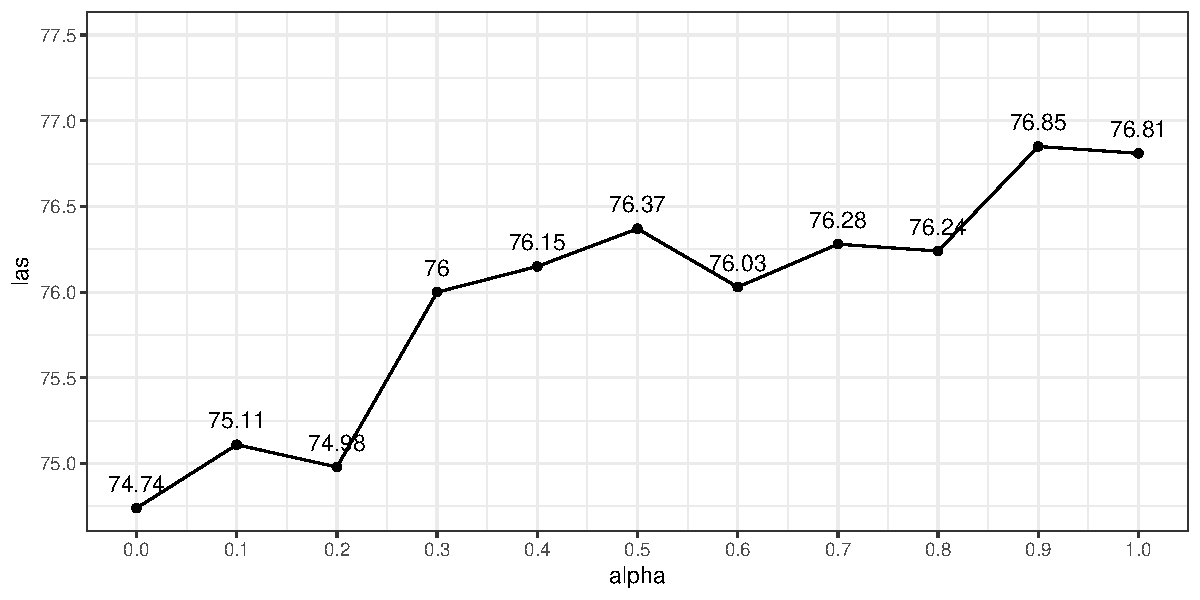
\includegraphics[width=\columnwidth]{graphics/alpha}
	\caption{The effect of $\alpha$ in distillation.}\label{fig:effect-alpha}
\end{figure}

We show the effect of $\alpha$ in Figure \ref{fig:effect-alpha}.
This figure shows that parsers with larger $\alpha$ achieves better performance than that with smaller $\alpha$.
This result shows that learning from the hard target in unnecessary.


%\paragraph{Effect of $\mathcal{T}$}
%
%\begin{figure}[t]
%	\centering
%	\includegraphics[width=\columnwidth]{graphics/temperature}
%	\caption{The effect of temperature $\alpha$.}\label{fig:effect-temp}
%\end{figure}

\paragraph{Results}

\begin{table}[t]
	\centering
	\small
	\begin{tabular}{rcc}
		\hline
		\it System & UAS & LAS \\
		\hline
		\newcite{ballesteros-EtAl:2016:EMNLP2016} & 79.25 & 74.17 \\
		\newcite{dyer-EtAl:2015:ACL-IJCNLP} & 77.90 & 72.95 \\
		Ensemble 20 & 82.80 & 78.69 \\
		Distill expert ($\alpha$=0.)& 81.22 & 76.98 \\
		Distill boltzmann ($\mathcal{T}$=1) & 81.55 & 77.32 \\
		\hline
	\end{tabular}
	\caption{The POS tagging result.}\label{tbl:parse-result}
\end{table}

%\subsection{Exploiting UD\_English}

%UD\_English as an important source of training data.
%\section{Model}
%We propose a new model


\section{Related Work}
%\yjcomment{related word is not finished.}
%\newcite{eisenstein:2013:NAACL-HLT} reviewed NLP approaches for analyzing text on social media, especially for tweets and showed that there are two major directions for NLP community to handle the tweets, including normalization and domain adaptation. He also pointed out that normalization can be problematic because precisely defining the normalization task is difficult. 
%
%\newcite{kong-EtAl:2014:EMNLP2014} argues that the Penn Treebank approach to annotation is poorly suited to more informal genres of text, as some of the annotation challenges for tweets,
%including token selection, multiword expressions, multiple roots, and structure within noun phrases diverge significantly from conventional approaches. 
%They believe that rapid, small scale annotation efforts performed by imperfectly-trained annotators should provide enough evidence to train an effective parser, given the rapidly changing nature of tweets~\cite{eisenstein:2013:NAACL-HLT}, the attested difficulties of domain adaptation for parsing~\cite{dred07}, and the expense of creating Penn Treebank-style annotations~\cite{penn93}. 
%Therefore, they build a new corpus of tweets (Tweebank), with conventions informed by the domain, using new syntactic annotations that can tackle all the forementioned problems annotated in a day by two dozen annotators, most of whom had only cursory training in the annotation scheme. Then, they modify the decoder of the TurboParser, a graph-based dependency parser, which is open-source and has been found to perform well on a range of parsing problems in different languages~\cite{turbo13} to adapt to the Tweebank dataset, and incorporate new features such as Brown Clusters and Penn Treebank features and changes to specification
%in the output space into TurboParser.
%
%Like ``mfw'' is usually followed by an adverbial clause and ``ima'' is usually followed by a clausal complement. 
%It is not reasonable to treat them in the same part-of-speech. 
%In this paper, when annotating the POS tagging for abbreviations, we first try to recover their original forms, then use the POS of the core-word as the POS for the abbreviation.
%Second, four special POS tags (S, L, M, Y) were designed to handle contraction words in Gimpel et al. \shortcite{Gimpel:2011:PTT:2002736.2002747}. Major concern of designing such tags is to minimize the effort of tokenization. 
%However, contractions of common nouns and pronouns are casted into the same category which increase the difficulty of distinguishing their syntactic function (say, there's and book'll are treated with the same syntactic function). What's more, only a small proportion of words can be categorized into these tags (2.7 \% in total), which cast a doubt of the usefulness of these certain tags. In this paper, we believe such contraction can be properly handled by tokenization module, so we suggest to tokenize the contraction word and annotate POS tag accordingly.
%Besides the contraction that be conventionally tokenized, tweets also witness a set of unconventional contraction like iv (I've), whatis (what is). In this paper, we follow the same idea of annotation abbreviation to handle the unconventional contractions and use the POS of core word of the original form as their POS.
%Third, special POS was designed to handle emoticon in Gimpel et al. \shortcite{Gimpel:2011:PTT:2002736.2002747}. However, in most cases, emoticon plays the same role as most of the symbolic tokens. In this paper, we follow the UD guideline to annotate the emoticon as symbol (SYM).
%At last, it’s arguable that some of the hashtags, URLs can work as a nominal in tweets. Whether treating them as the same part-of-speech or different ones according to their context is an open question. A preliminary survey on the standard UD English data shows that URL, email address are all tagged as the foreign language (X), so we also tag them as X and leave the disambiguation of their syntactic function to the annotation of parse tree.

\section{Conclusion}

\bibliography{shortdb}
\bibliographystyle{acl_natbib}
\end{document}
